\documentclass[]{article}
\usepackage{lmodern}
\usepackage{amssymb,amsmath}
\usepackage{ifxetex,ifluatex}
\usepackage{fixltx2e} % provides \textsubscript
\ifnum 0\ifxetex 1\fi\ifluatex 1\fi=0 % if pdftex
  \usepackage[T1]{fontenc}
  \usepackage[utf8]{inputenc}
\else % if luatex or xelatex
  \ifxetex
    \usepackage{mathspec}
  \else
    \usepackage{fontspec}
  \fi
  \defaultfontfeatures{Ligatures=TeX,Scale=MatchLowercase}
\fi
% use upquote if available, for straight quotes in verbatim environments
\IfFileExists{upquote.sty}{\usepackage{upquote}}{}
% use microtype if available
\IfFileExists{microtype.sty}{%
\usepackage{microtype}
\UseMicrotypeSet[protrusion]{basicmath} % disable protrusion for tt fonts
}{}
\usepackage[margin=1in]{geometry}
\usepackage{hyperref}
\hypersetup{unicode=true,
            pdftitle={Study on the leap year effect},
            pdfborder={0 0 0},
            breaklinks=true}
\urlstyle{same}  % don't use monospace font for urls
\usepackage{natbib}
\bibliographystyle{unsrt}
\usepackage{longtable,booktabs}
\usepackage{graphicx,grffile}
\makeatletter
\def\maxwidth{\ifdim\Gin@nat@width>\linewidth\linewidth\else\Gin@nat@width\fi}
\def\maxheight{\ifdim\Gin@nat@height>\textheight\textheight\else\Gin@nat@height\fi}
\makeatother
% Scale images if necessary, so that they will not overflow the page
% margins by default, and it is still possible to overwrite the defaults
% using explicit options in \includegraphics[width, height, ...]{}
\setkeys{Gin}{width=\maxwidth,height=\maxheight,keepaspectratio}
\IfFileExists{parskip.sty}{%
\usepackage{parskip}
}{% else
\setlength{\parindent}{0pt}
\setlength{\parskip}{6pt plus 2pt minus 1pt}
}
\setlength{\emergencystretch}{3em}  % prevent overfull lines
\providecommand{\tightlist}{%
  \setlength{\itemsep}{0pt}\setlength{\parskip}{0pt}}
\setcounter{secnumdepth}{5}
% Redefines (sub)paragraphs to behave more like sections
\ifx\paragraph\undefined\else
\let\oldparagraph\paragraph
\renewcommand{\paragraph}[1]{\oldparagraph{#1}\mbox{}}
\fi
\ifx\subparagraph\undefined\else
\let\oldsubparagraph\subparagraph
\renewcommand{\subparagraph}[1]{\oldsubparagraph{#1}\mbox{}}
\fi

%%% Use protect on footnotes to avoid problems with footnotes in titles
\let\rmarkdownfootnote\footnote%
\def\footnote{\protect\rmarkdownfootnote}

%%% Change title format to be more compact
\usepackage{titling}

% Create subtitle command for use in maketitle
\newcommand{\subtitle}[1]{
  \posttitle{
    \begin{center}\large#1\end{center}
    }
}

\setlength{\droptitle}{-2em}
  \title{Study on the leap year effect}
  \pretitle{\vspace{\droptitle}\centering\huge}
  \posttitle{\par}
  \author{}
  \preauthor{}\postauthor{}
  \date{}
  \predate{}\postdate{}

\usepackage{booktabs}
\usepackage{longtable}
\usepackage{array}
\usepackage{multirow}
\usepackage[table]{xcolor}
\usepackage{wrapfig}
\usepackage{float}
\usepackage{colortbl}
\usepackage{pdflscape}
\usepackage{tabu}
\usepackage{threeparttable}
\usepackage[normalem]{ulem}

\usepackage{mathtools}

\usepackage{amsthm}
\newtheorem{theorem}{Theorem}[section]
\newtheorem{lemma}{Lemma}[section]
\theoremstyle{definition}
\newtheorem{definition}{Definition}[section]
\newtheorem{corollary}{Corollary}[section]
\newtheorem{proposition}{Proposition}[section]
\theoremstyle{definition}
\newtheorem{example}{Example}[section]
\theoremstyle{definition}
\newtheorem{exercise}{Exercise}[section]
\theoremstyle{remark}
\newtheorem*{remark}{Remark}
\newtheorem*{solution}{Solution}
\begin{document}
\maketitle

{
\setcounter{tocdepth}{2}
\tableofcontents
}
\section{Introduction}\label{introduction}

In order to keep the calendar year synchronized with the astronomical
year, the calendar year can contains one additional day in February. It
happens almost every four years\footnote{More precisely it happens in
  years which are multiples of four, with the exception of years
  divisible by 100 but not by 400.} and a year that contains 29 days in
February is called a leap year (the next leap year is in 2020). The leap
year has to be taken into account in the interpretation of some
economical indicators. Indeed, one additional working day in February
implies one additional day of production and therefore an increase of
the production, even if the productivity has remained constant. To
compare changes within a year or between months of different years, lots
of economical series are seasonal adjusted and correcting for working
days, and so for leap year. This is for example the case of the
industrial production indexes.

Not all the time series are affected by leap years. For example, when
the Labor Force Survey asks respondent for their employment status over
a particular week, unemployment estimates are not likely to be affected
by leap years. Nevertheless, when time series are likely to be affected
by leap years, it may not be possible to correctly estimate it for
multiple reasons:

\begin{itemize}
\tightlist
\item
  If the leap year effect is too weak to be estimate. For instance, it
  can be the case when production is measured in ``quantities produced''
  as for the French production index relate to airplane airframes.
  Indeed, an additional day in February may not implies an additional
  number of finished planes during the month and therefore the leap year
  may not be statistically significant. For the similar reason it may be
  difficult to estimate the leap year effect in quarterly series.\\
\item
  If the series span is too short to estimate a leap year effect because
  it can conduce to misleading results. Indeed, if the series span
  doesn't contain any leap year it makes no sense to estimate its
  effect. However, if the series span only contains one leap year, is it
  enough to correctly estimate its effect? If not, how many observations
  do we need to have a robust estimation? Another question comes arise:
  does the leap year effect is similar to all data, as it would expect
  to be?
\end{itemize}

Is to those three questions that we aim to respond. The data use are
monthly and correspond to the turnover indexes in industry, services and
in wholesale and retail trail and the industrial production indexes of
the European Union members\footnote{The \emph{sts\_intv\_m},
  \emph{sts\_setu\_m}, \emph{sts\_sepr\_m} and \emph{sts\_inpr\_m},
  datasets of Eurostat.}. Series are study at three levels of the NACE
Rev 2 (two, three and four digits) and are retains only if more than 12
years of data is available: 2 198 series are examine. For all of them,
the leap year effect is economically explainable.

\section{How and when carry out the leap year
adjustment?}\label{how-and-when-carry-out-the-leap-year-adjustment}

\subsection{The leap year adjustment}\label{subsect:lyadj}

The leap year adjustment is usually made by two different methods:

\begin{itemize}
\tightlist
\item
  Adding an explanatory variable in a regression model with ARIMA times
  series errors (regARIMA model). The leap year regressor (\(L_t\)) used
  in X13ARIMA-SEATS is defined as: \[
  L_t = \begin{cases}
  0.75 & \text{ in February during leap years} \\
  -0.25  & \text{ in February during non leap years} \\
  0 & \text{ for all other months}
  \end{cases}
  \] Therefore, the leap year effect can be defined as the estimate
  value of the coefficient of the leap year regressor. This value
  depends in particular on if series are assumed that unobserved
  components of the time series combine multiplicatively or additively;
  it can also depends, to a lesser extent, on the other components of
  the regARIMA model (for example in the case of model failures).\\
\item
  Correcting values prior to modelling multiplying by a fixed
  proportion: \[\begin{cases}
  \frac{28.25}{29} & \text{ in February during leap years} \\
  \frac{28.25}{28}  & \text{ in February during non leap years} \\
  1 & \text{ for all other months}
  \end{cases}\] In the case of multiplicative models, this is equivalent
  to adding a leap year regressor if and only if the coefficient is
  approximately equal to 0.035 (which is the approximate value expected
  in the multiplicative model; see appendix \ref{sect:appendix})
  \citep{bell1992lengthmonthadj}. This isn't true for additive models.
\end{itemize}

\subsection{When does the leap year adjustment should be
done?}\label{when-does-the-leap-year-adjustment-should-be-done}

According to the ESS Guidelines on seasonal adjustment
\citep{eurostat2015guidelines}, the leap year adjustment should only be
done for time series for which there is an economic explanation and a
statistical evidence. This is for example what is done by the Office for
National Statistics of the United Kingdom \citep{ons2016noteonleapyear}.

In this study, there is an economic explanation for all time series.
Therefore adjusting from the leap year effect make sense and the
statistical evidence will then be tested.

\section{From the regARIMA model to the study of the convergence of the
leap year
estimation}\label{from-the-regarima-model-to-the-study-of-the-convergence-of-the-leap-year-estimation}

\subsection{The regARIMA model}\label{subsect:regarima}

In this study, all time series are working days and leap years adjust
(even if there isn't statistical evidence) and the estimation is done in
the presence of possibly several types of outlier. In the case of
additive model, the following regARIMA model is used:

\begin{equation} 
Y_t = \beta_0 L_t + \beta_1 WD_t + 
\underbrace{\sum_{i}\gamma_iO_{i,t}}_{\mathclap{\text{possibly absent}}} + \varepsilon_t
 \label{eq:model}
\end{equation}

where \(Y_t\) is the observed time series, \(L_t\) the leap year
regressor defined in the section \ref{subsect:lyadj}, \(WD_t\) the
working day regressor, \(O_{i,t}\) possibles outliers and
\(\varepsilon_t\) has mean zero and follows an airline ARIMA model (an
ARIMA(0,1,1)(0,1,1)).

In the case of multiplicative combination, a logarithm transformation is
applied to the observed series and then modelled additively: the same
model than \eqref{eq:model} is used but replacing \(Y_t\) by
\(\log (Y_t)\):

\begin{equation} 
\log(Y_t) = \beta_0 L_t + \beta_1 WD_t + \sum_{i}\gamma_iO_{i,t} + \varepsilon_t
 \label{eq:model-log}
\end{equation}

The leap year effect is thus \(\beta_0\). In the multiplicative model
the value we would expect for \(\beta_0\) is closed to 0.035. However
estimates values of \(\beta_0\) can deviate from 0.035 due to various
model failures such as presence of autocorrelation of heteroskedasticity
on regARIMA residuals (since this bias the estimates of the regression
parameters). Because all the time series used in this study are indexes
of base 100, we could also assume that value we would expect for
\(\beta_0\) in the multiplicative model is closed to 3.5 (this is the
case for almost all series study here).

For all time series the methodology described as followed is used to
study the estimation of the leap year effect:

\begin{itemize}
\tightlist
\item
  First, we study each series throughout the entire sample in order to
  determine the decomposition of the times series (multiplicative or
  additive).\\
\item
  Then, we identify a regARIMA model (detecting outliers) and estimate
  it from the beginning of the time series with a four years span fixing
  the decomposition (determine in the first step)\footnote{Four years
    are needed to have at least one leap year.}. In the same way we
  re-identify and re-estimate the model for each additional date to the
  end of the sample (always from the beginning of the time series).
\end{itemize}

\subsection{Study of the convergence of the leap year
estimation}\label{subsect:etud-conv}

In the study we defined the \emph{time convergence} of the leap year
estimation as the elapsed time required for the leap year estimation to
remain statistically significant and not statistically different from
the last estimation (or from the expected value defined in
\ref{subsect:regarima}). That is to say that the \emph{time convergence}
is the the elapsed time required for the decision to perform a leap year
adjustment to remain permanent and to the estimation to stabilize.

For instance, taking a times series starting in January 2000 and ending
in December 2015, a time convergence equal to 8 years means that if we
re-identify and re-estimate the model from January 2000 to any date
after January 2008:

\begin{itemize}
\tightlist
\item
  the leap year is statistically significant;\\
\item
  the leap year is not statistically different from value estimate from
  January 2000 to December 2015 (or from the expected value defined in
  \ref{subsect:regarima}).
\end{itemize}

When the leap year estimation isn't statistically significant, we then
consider that we don't have convergence and so we don't have any time
convergence.

\section{Results}\label{results}

\subsection{Preliminary study}\label{preliminary-study}

Almost all series have converged to the expected value (92.7\%; table
\ref{tab:schema-cv}), whether in a multiplicative or an additive model.
Only 3 series can't be force to multiplicative model (because some data
are too closed to zero) and it affects negligently the significativity
of the leap year effects and it's convergence to the expected value. So,
in order to make further comparison easier, all series will be forced to
multiplicative decomposition\footnote{Same results are found without
  forcing multiplicative decomposition.} and we will study the leap year
convergence to the value of 0.035 (for which adding a regressor is
equivalent to pre-adjusting the initial times series to correct from the
leap year effect).

\begin{table}[!h]

\caption{\label{tab:schema-cv}Statistics on convergence of the leap year (LY) effect by decomposition}
\centering
\begin{tabular}[t]{l>{\centering\arraybackslash}p{2.5cm}>{\centering\arraybackslash}p{2.5cm}>{\centering\arraybackslash}p{2.5cm}c}
\toprule
\multicolumn{1}{c}{ } & \multicolumn{2}{c}{As converged to the expected value\textsuperscript{a}} & \multicolumn{2}{c}{The LY coefficient is significant} \\
\cmidrule(l{2pt}r{2pt}){2-3} \cmidrule(l{2pt}r{2pt}){4-5}
 & Yes & No & Yes & No\\
\midrule
\addlinespace[0.3em]
\multicolumn{5}{l}{\textbf{Initial decomposition\textsuperscript{b}}}\\
\hspace{1em}Additive & 676 & 70 & 235 & 511\\
\hspace{1em}Multiplicative & 1361 & 91 & 429 & 1023\\
\addlinespace[0.3em]
\multicolumn{5}{l}{\textbf{Forced to multiplicative\textsuperscript{c}}}\\
\hspace{1em}Initially additive & 673 & 70 & 239 & 504\\
\bottomrule
\multicolumn{5}{l}{\textbf{Notes:}  Tests are done with 5\% significance level;}\\
\multicolumn{5}{l}{\textsuperscript{a} 0.035 for multiplicative decomposition and 3.5 for additive decomposition;}\\
\multicolumn{5}{l}{\textsuperscript{b} Indentified estimating the model throughout the entire sample;}\\
\multicolumn{5}{l}{\textsuperscript{c} 3 series can't be forced to multiplicative decomposition.}\\
\end{tabular}
\end{table}

\begin{table}[!h]

\caption{\label{tab:res-pb}Statistics on regARIMA residuals, forcing the multiplicative decomposition}
\centering
\begin{tabular}[t]{l>{\centering\arraybackslash}p{2cm}>{\centering\arraybackslash}p{2cm}}
\toprule
\multicolumn{1}{c}{ } & \multicolumn{2}{c}{The LY\textsuperscript{*} coefficient is significant} \\
\cmidrule(l{2pt}r{2pt}){2-3}
 & Yes & No\\
\midrule
\addlinespace[0.3em]
\multicolumn{3}{l}{\textbf{RegARIMA residuals are autocorrelated or heteroskedastics}}\\
\hspace{1em}As converged to the expected value & 285 & 564\\
\hspace{1em}Asn't converged to the expected value & 28 & 43\\
\addlinespace[0.3em]
\multicolumn{3}{l}{\textbf{RegARIMA residuals are correct}}\\
\hspace{1em}As converged to the expected value & 326 & 859\\
\hspace{1em}Asn't converged to the expected value & 29 & 61\\
\bottomrule
\multicolumn{3}{l}{\textbf{Notes:}  Tests on residuals are done with 1\% significance level;}\\
\multicolumn{3}{l}{Significativity test done with 5\% significance level.}\\
\multicolumn{3}{l}{\textsuperscript{*} LY=Leap year}\\
\end{tabular}
\end{table}

Results must be carefully considered when regARIMA residuals are
autocorrelated or heteroskedastics. Indeed, in this case the estimated
variance of the leap year coefficient is biased (the estimated
coefficient can also be biased) and so tests on time convergence are
wrong. This is the case for 920 series (table \ref{tab:res-pb}). On the
2 195 series examined, only 14.3\% have a leap year statistically
significant with correct regARIMA residuals. That is to say that,
studying the time series throughout the entire sample, we would have
doubtlessly proceed to the leap year adjustment for only 14.3\% of them!

\subsection{Study of the time
convergence}\label{study-of-the-time-convergence}

\begin{table}[!h]

\caption{\label{tab:conv-stats}Quantiles on time convergence (in years) of the leap year coefficient to 0.035 with a free ARIMA model}
\centering
\begin{tabular}[t]{lcccccc}
\toprule
 & Minimum & 65\% & 70\% & 80\% & 90\% & Maximum\\
\midrule
\addlinespace[0.3em]
\multicolumn{7}{l}{\textbf{RegARIMA residuals are correct}}\\
\hspace{1em}The LY coefficient is significant & 4.0 & 4.0 & 4.0 & 5.2 & 10.2 & 26.3\\
\hspace{1em}The LY coefficient isn't significant & 4.0 & 4.0 & 4.0 & 5.2 & 10.5 & 26.6\\
\addlinespace[0.3em]
\multicolumn{7}{l}{\textbf{RegARIMA residuals are autocorrelated or heteroskedastics}}\\
\hspace{1em}The LY coefficient is significant & 4.0 & 4.0 & 4.0 & 6.3 & 13.6 & 26.5\\
\hspace{1em}The LY coefficient isn't significant & 4.0 & 4.0 & 4.5 & 8.1 & 14.5 & 26.9\\
\bottomrule
\multicolumn{7}{l}{\textbf{Notes:}  Tests on residuals are done with 1\% significance level;}\\
\multicolumn{7}{l}{Significativity test done with 5\% significance level.}\\
\multicolumn{7}{l}{\textbf{How to read it:}  For 80\% of the times series for which regARIMA residuals are correct and}\\
\multicolumn{7}{l}{the leap year statistically significant, it takes less than 5.2 years to converge to 0.035.}\\
\end{tabular}
\end{table}

The elapsed time for the leap year estimation to remain not
significantly different from 0.035 is very short (table
\ref{tab:conv-stats}): it takes less than 6 years for 80\% of the time
series. However, the elapsed time for the leap year estimation to remain
significant is much longer (figure \ref{fig:violin-conv-signif}): more
than 10 years for 75\% of the 624 times series for which the leap year
is statistically significant. That implies a long time convergence of
the leap year estimation (figure \ref{fig:violin-time-conv}).

\begin{figure}[!hbt]
\centering
\caption{Time for the leap year coefficient to remain significantly different from zero}
\label{fig:violin-conv-signif}
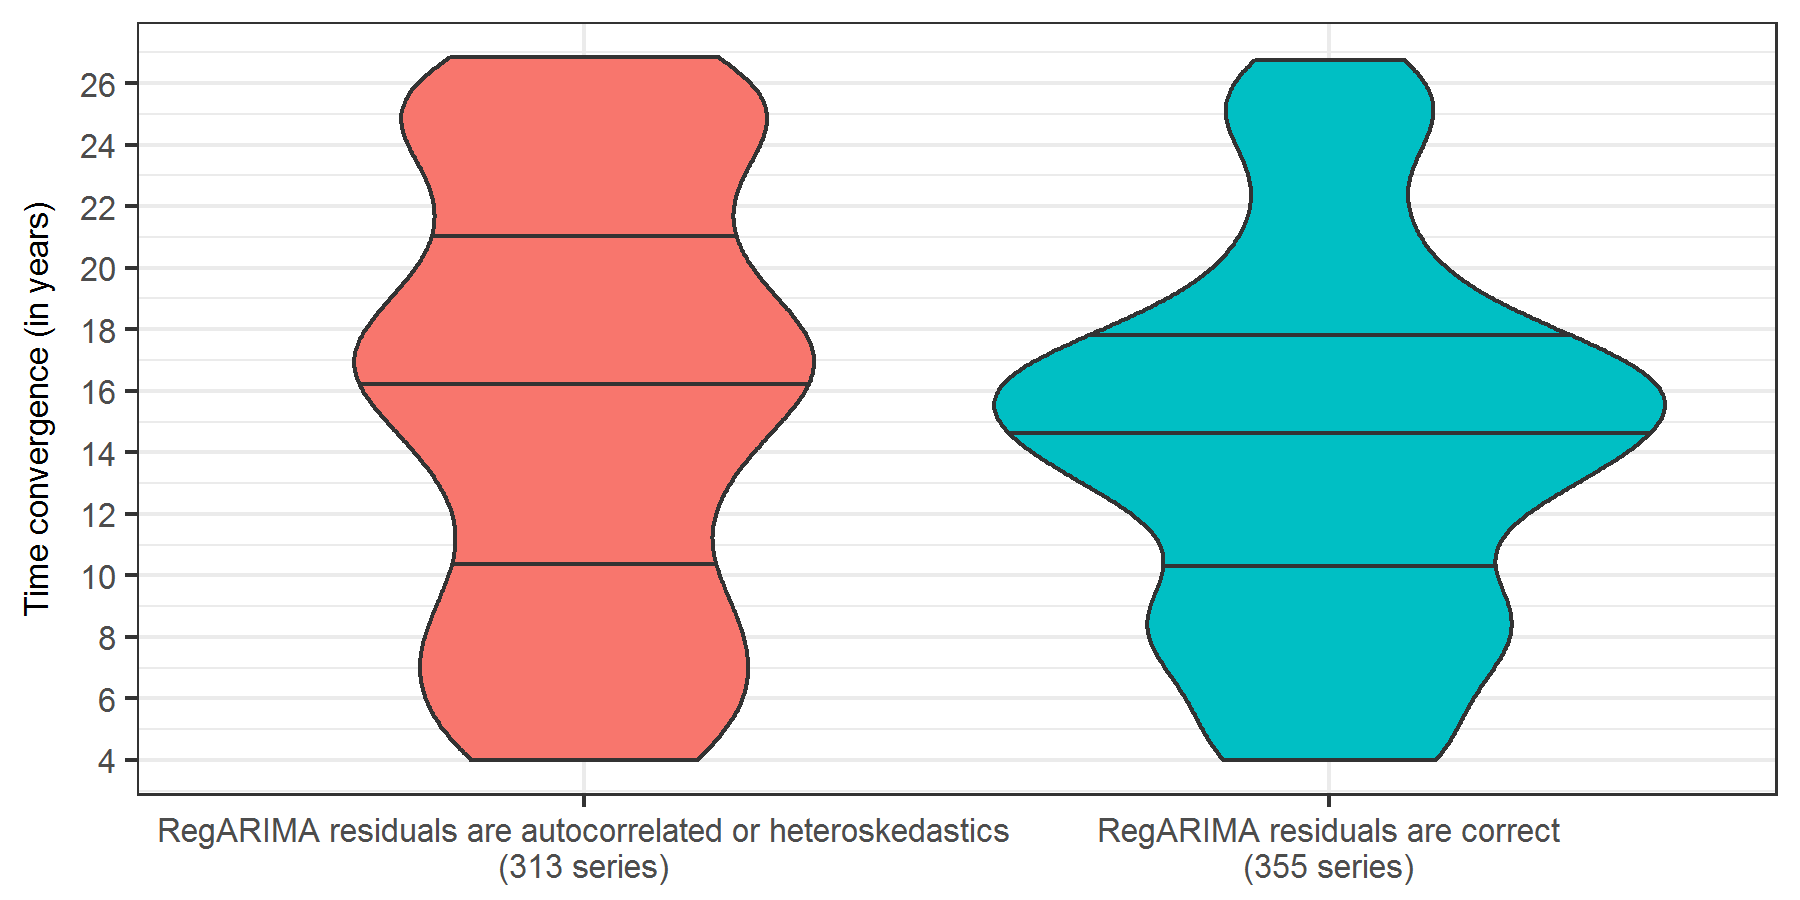
\includegraphics{img/violin_conv_signif.png}
\footnotesize

\textbf{How to read it:} Violin plots represent a rotated kernel density plot, horizontal lines representing quartiles.
\end{figure}

\begin{figure}[!hbt]
\centering
\caption{Time convergence of the leap year estimation}
\label{fig:violin-time-conv}
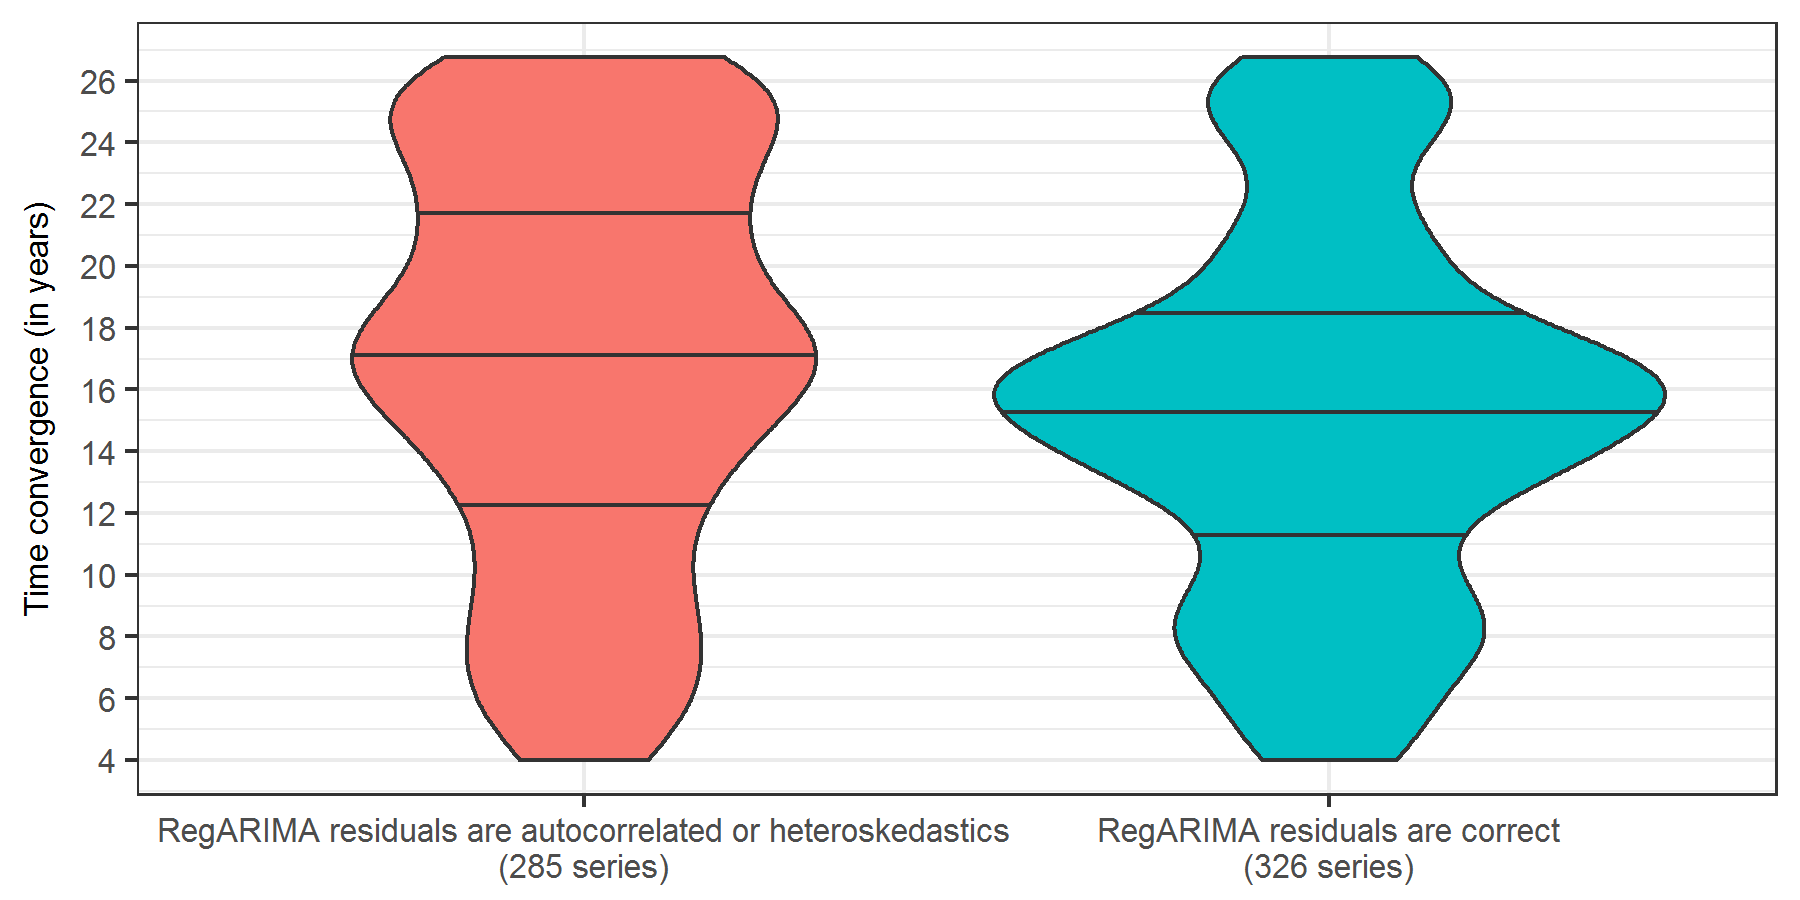
\includegraphics{img/violin_time_conv.png}
\footnotesize

\textbf{How to read it:} Violin plots represent a rotated kernel density plot, horizontal lines representing quartiles.
\end{figure}

\subsection{Estimate value of the leap year
coefficient}\label{estimate-value-of-the-leap-year-coefficient}

Until there, we have study the convergence of the leap year estimation
without looking at the estimate value of the coefficient. Even if it
isn't significantly different from the value of 0.035 for almost all
series, the regARIMA estimation can lead to senseless negative values
(graph \ref{fig:violin-conv-coef}) or questionable high coefficients
(above 0.1: it means that the production in February has increased by
more than 7.8\% just because of the additional day).

\begin{figure}[!hbt]
\centering
\caption{Distribution of the estimate values of the leap year coefficient}
\label{fig:violin-conv-coef}
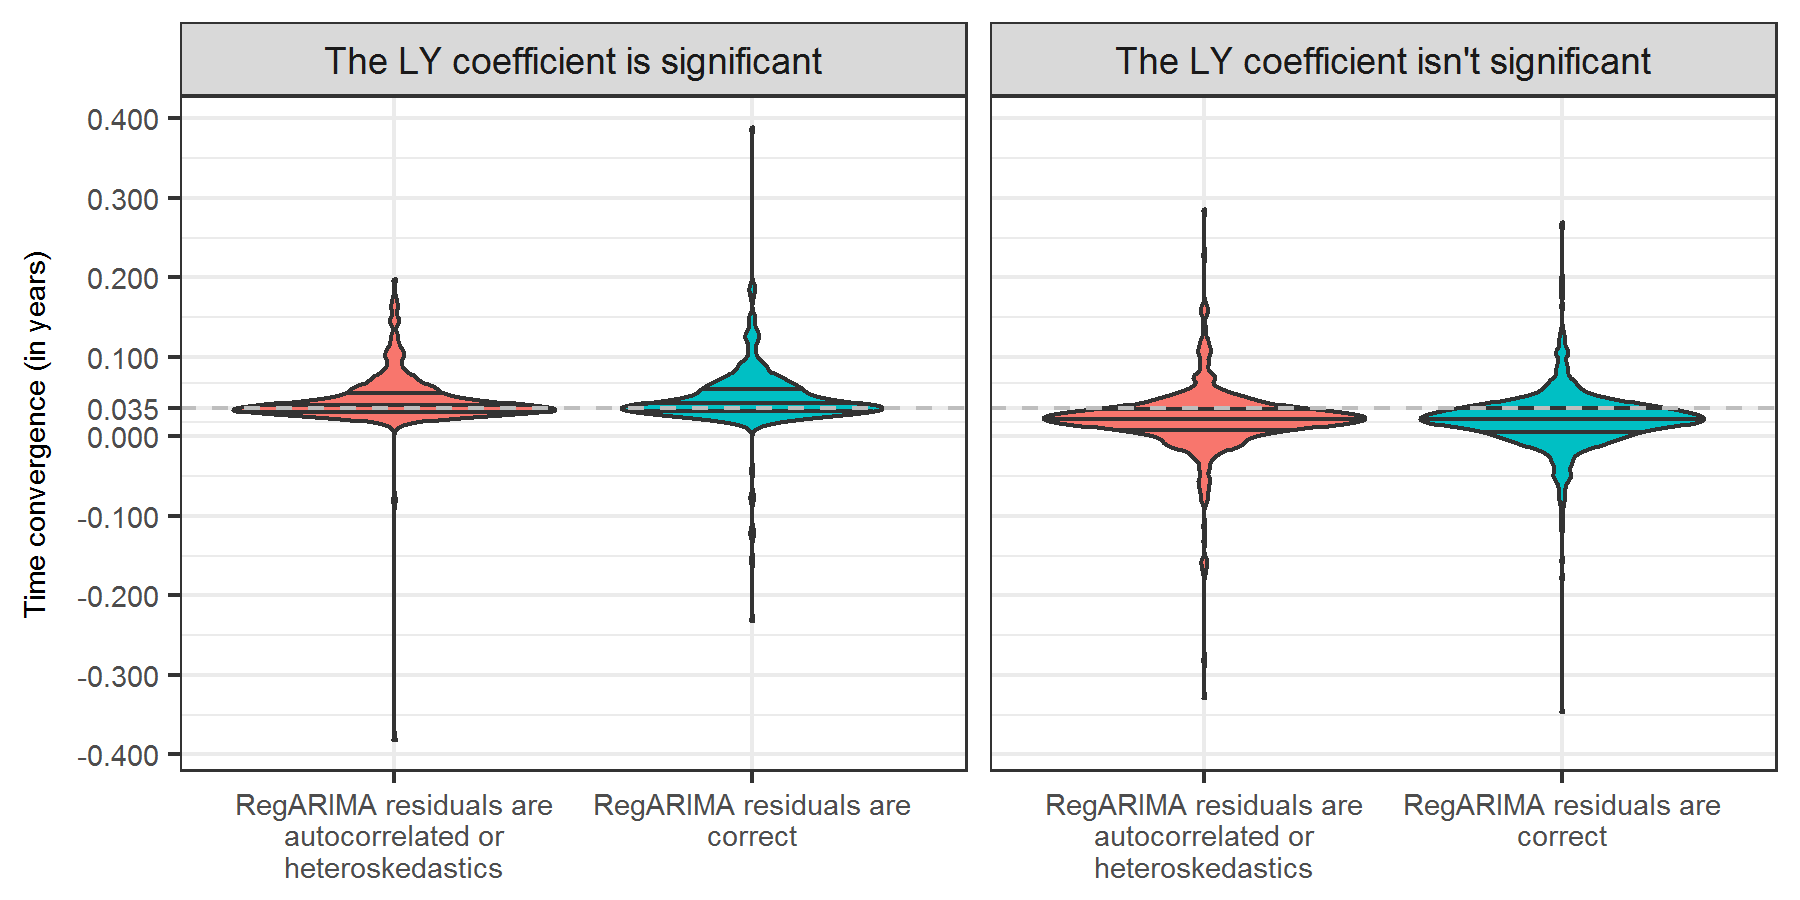
\includegraphics{img/violin_conv_coef.png}
\footnotesize

\textbf{How to read it:} Violin plots represent a rotated kernel density plot, horizontal lines representing quartiles.
\end{figure}

\section{Changing the ARIMA model}\label{changing-the-arima-model}

In the regARIMA model (equations \eqref{eq:model} and \eqref{eq:model-log})
we assume that errors have mean zero and follow an airline ARIMA model.
This hypothesis can be discussed, in particular regarding to the
presence of autocorrelation or heteroskedasticity. In this section we
study the time convergence of the leap year estimation but with a free
ARIMA model: the model is identified by the estimation throughout the
entire sample and is use for each estimation (see section
\ref{subsect:etud-conv}). Although it reduce the number of time series
for which regARIMA residuals aren't autocorrelated or heteroskedastics
(table \ref{tab:res-pb-free-arima}), it doesn't change the previous
results. While the elapsed time for the leap year to remain not
significantly different from 0.035 is usually short (table
\ref{tab:conv-stats-free-arima}), it needs a long period to remain
statistically significant (figure
\ref{fig:violin-conv-signif-arima-free}) and so a long time convergence.

\begin{table}[!h]

\caption{\label{tab:res-pb-free-arima}Statistics on regARIMA residuals, forcing the multiplicative decomposition with a free ARIMA model}
\centering
\begin{tabular}[t]{l>{\centering\arraybackslash}p{2cm}>{\centering\arraybackslash}p{2cm}}
\toprule
\multicolumn{1}{c}{ } & \multicolumn{2}{c}{The LY\textsuperscript{*} coefficient is significant} \\
\cmidrule(l{2pt}r{2pt}){2-3}
 & Yes & No\\
\midrule
\addlinespace[0.3em]
\multicolumn{3}{l}{\textbf{RegARIMA residuals are autocorrelated or heteroskedastics}}\\
\hspace{1em}As converged to the expected value & 224 & 486\\
\hspace{1em}Asn't converged to the expected value & 31 & 35\\
\addlinespace[0.3em]
\multicolumn{3}{l}{\textbf{RegARIMA residuals are correct}}\\
\hspace{1em}As converged to the expected value & 377 & 936\\
\hspace{1em}Asn't converged to the expected value & 34 & 72\\
\bottomrule
\multicolumn{3}{l}{\textbf{Notes:}  Tests on residuals are done with 1\% significance level;}\\
\multicolumn{3}{l}{Significativity test done with 5\% significance level.}\\
\multicolumn{3}{l}{\textsuperscript{*} LY=Leap year}\\
\end{tabular}
\end{table}

\begin{table}[!h]

\caption{\label{tab:conv-stats-free-arima}Quantiles on time convergence (in years) of the leap year coefficient to 0.035 with a free ARIMA model}
\centering
\begin{tabular}[t]{lcccccc}
\toprule
 & Minimum & 65\% & 70\% & 80\% & 90\% & Maximum\\
\midrule
\addlinespace[0.3em]
\multicolumn{7}{l}{\textbf{RegARIMA residuals are correct}}\\
\hspace{1em}The LY coefficient is significant & 4.0 & 4.0 & 4.2 & 6.1 & 11.2 & 26.3\\
\hspace{1em}The LY coefficient isn't significant & 4.0 & 4.0 & 4.1 & 5.9 & 11.0 & 26.4\\
\addlinespace[0.3em]
\multicolumn{7}{l}{\textbf{RegARIMA residuals are autocorrelated or heteroskedastics}}\\
\hspace{1em}The LY coefficient is significant & 4.0 & 4.8 & 5.9 & 8.2 & 16.1 & 26.5\\
\hspace{1em}The LY coefficient isn't significant & 4.0 & 4.7 & 5.7 & 8.8 & 15.2 & 26.1\\
\bottomrule
\multicolumn{7}{l}{\textbf{Notes:}  Tests on residuals are done with 1\% significance level;}\\
\multicolumn{7}{l}{Significativity test done with 5\% significance level.}\\
\multicolumn{7}{l}{\textbf{How to read it:}  For 80\% of the times series for which regARIMA residuals are correct and}\\
\multicolumn{7}{l}{the leap year statistically significant, it takes less than 6.1 years to converge to 0.035.}\\
\end{tabular}
\end{table}

\begin{figure}[!hbt]
\centering
\caption{Time for the leap year coefficient to remain significantly different from zero with a free ARIMA model}
\label{fig:violin-conv-signif-arima-free}
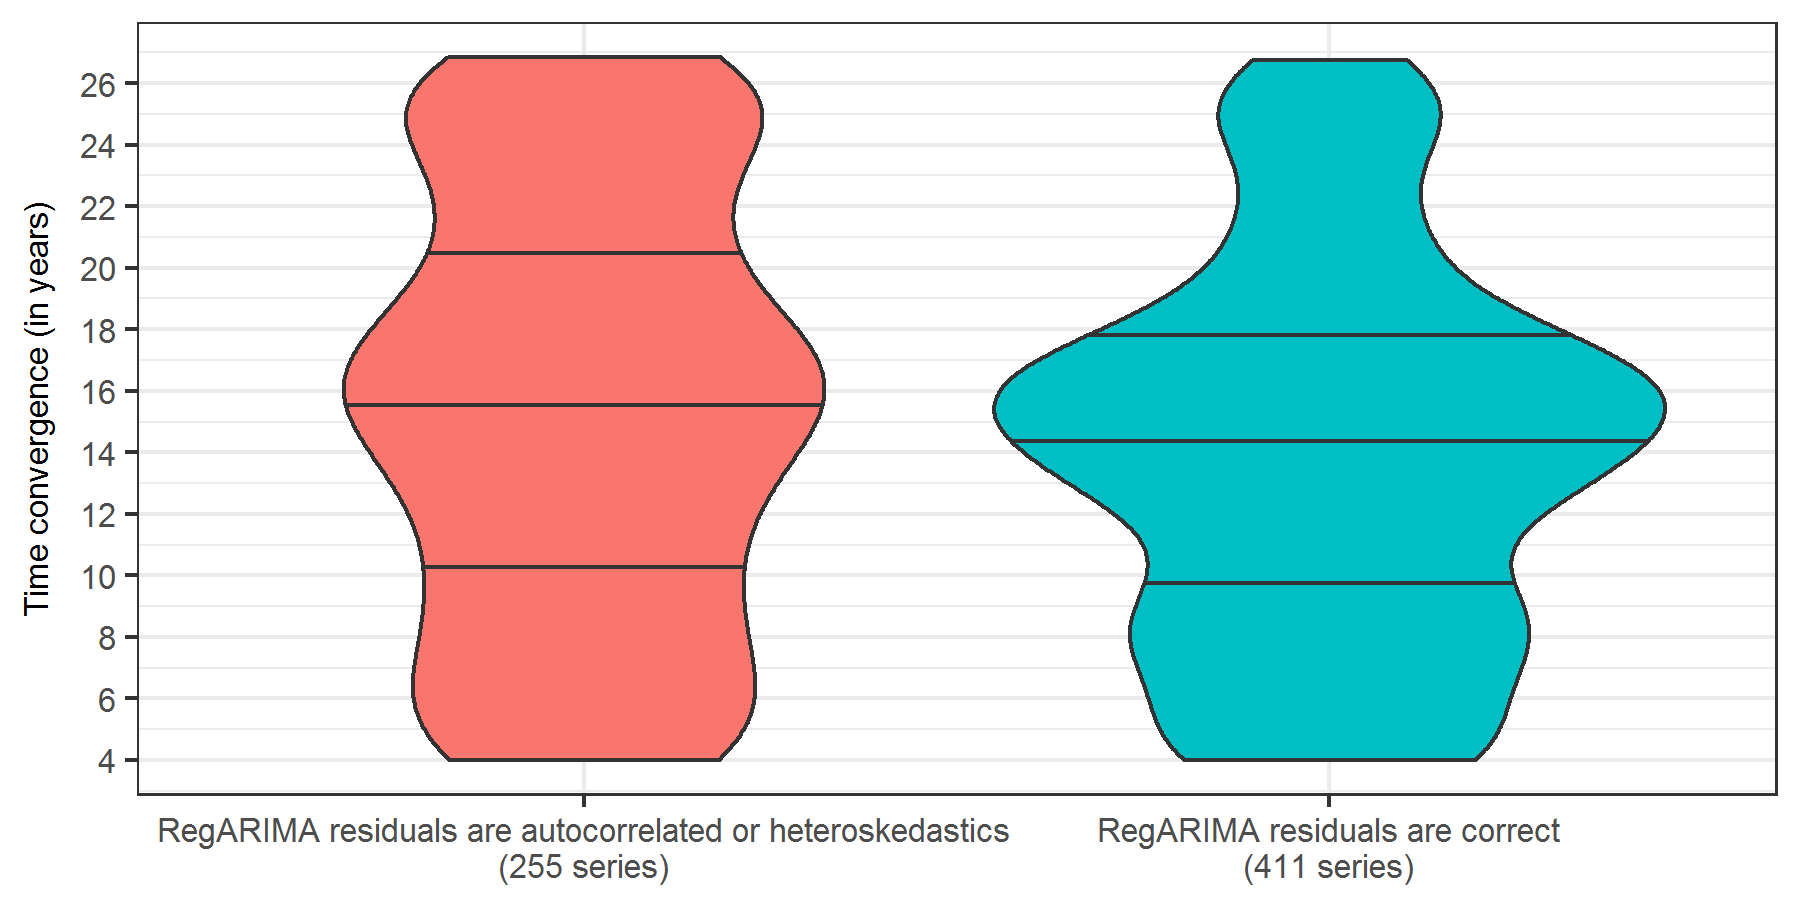
\includegraphics{img/violin_conv_signif_arima_free.png}
\footnotesize

\textbf{How to read it:} Violin plots represent a rotated kernel density plot, horizontal lines representing quartiles.
\end{figure}

\section{Conclusions}\label{conclusions}

The leap year adjustment performed including in the regARIMA model must
be done carefully, especially with short time series. Indeed, the time
convergence of the leap year estimation is quite long (more than 10
years for most series): for short time series the estimation may not be
stable. So we may erroneously conclude that the leap year is
statistically significant and vice versa.

Conversely, it is not recommended to perform an adjustment for time
series exceeding twenty years of length since it may produce sub-optimal
results \citep{eurostat2015guidelines}. For long time series it's thus
not recommended to use a regARIMA model to correct from the leap year
effect.

Moreover the regARIMA model can lead to strange estimate leap year
coefficient (and so to suspicious leap year adjustment) surely due to
model failures.

For all time series where the leap year is economically explainable,
correcting values from the leap year effect prior to modelling could be
preferred. For multiplicative decomposition it's equivalent to adding a
regressor in the regARIMA model and it avoids facing to model failures,
suspicious adjustment or convergence problems. For additive
decomposition it seems preferable due to the long time convergence which
could lead to wrong decisions.

\appendix

\section{Alternative approaches to leap year
adjustment}\label{sect:appendix}

Description of Bell's paper.

\bibliography{biblio.bib}


\end{document}
